%\documentclass[preprint,tightenlines,showpacs,showkeys,floatfix,
%nofootinbib,superscriptaddress,fleqn]{revtex4} 
\documentclass[floatfix,nofootinbib,superscriptaddress,fleqn,preprint]{revtex4} 
%\documentclass[aps,epsfig,tightlines,fleqn]{revtex4}
\usepackage[utf]{kotex}
\usepackage[HWP]{dhucs-interword}
\usepackage[dvips]{color}
\usepackage{graphicx}
\usepackage{bm}
%\usepackage{fancyhdr}
%\usepackage{dcolumn}
\usepackage{defcolor}
\usepackage{amsmath}
\usepackage{amsfonts}
\usepackage{amssymb}
\usepackage{amscd}
\usepackage{amsthm}
\usepackage[utf8]{inputenc}
 \usepackage{setspace}
%\pagestyle{fancy}

\begin{document}

\title{\Large 2022년 1학기 물리학 I: Quiz 8}
\author{김현철\footnote{Office: 5S-436D (면담시간 매주
    화요일-16:00$\sim$20:00)}} 
\email{hchkim@inha.ac.kr}
\affiliation{Hadron Theory Group, Department of Physics,
Inha University, Incheon 22212, Republic of Korea }
\date{Spring semester, 2022}


\vspace{1.cm}
\begin{abstract}
\noindent \textbf{ {\color{red}주의}: \color{blue} 단 한 번의 부정행위도 절대
  용납하지 않습니다. 적발 시, 학점은 F를 받게 됨은 물론이고,
  징계위원회에 회부합니다. One strike out임을 명심하세요.}\\
\\
문제는 다음 쪽부터 나옵니다.  \\ \\
{\bf Date:} 2022년 3월 28일 (월) 15:30-16:15 
\\
{\bf 학번:} \hspace{4cm}
{\bf 이름:} 

\end{abstract}
\maketitle

\noindent {\bf 문제 1 [20pt]}
가득 찬 화물용 승강기가 천천히 움직이고
있다. 이 승강기의 질량은 $1\,200$ kg이다. 정지상태에서 출발하여 3.0분
동안 54 m를 올라가서 정지하였다. 승강이 대응추의 질량이 950 kg밖에
되지 않으므로 모터의 도움이 필요하다. 케이블을 통해 모터에 작용하는
평균 일률은 얼마인가?

\newpage

{\color{gray} [문제 풀이 쪽]}

\newpage 

\noindent {\bf 문제 2 [20pt]}
그림~\ref{fig:2}과 같이 얼음덩어리가 경사각이 $\theta=50^\circ$이고
쓸림이 없는 경사면을 미끄러져 내려오고 있다. 이를 막기 위하여 크기가
50 N인 힘 $\vec{F}_r$로 얼음덩어리에 연결된 출을 잡아당기고
있다. 얼음덩어리가 경사면을 따라 거리 $d=0.50$ m만큼 미끄러져 내려왔을
때 운동에너지가 80 J 증가하였다. 만일 줄을 잡아당기지 않았다면
운동에너지는 얼마만큼 더 증가하겠는가?
\begin{figure}[ht]
  \centering
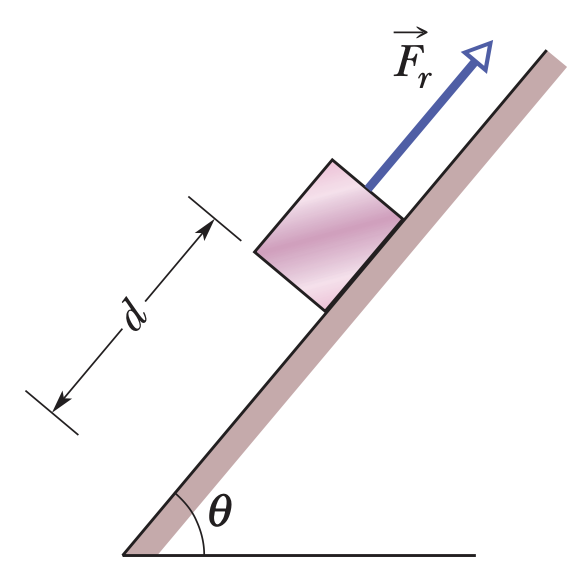
\includegraphics[scale=0.5]{Qfig8-2-20220328.png}
  \caption{문제 2}
  \label{fig:2}
\end{figure}
\newpage

{\color{gray} [문제 풀이 쪽]}

\newpage 

\noindent {\bf 문제 3 [60pt]}
그림~\ref{fig:3}는 질량 $m=0.032$ kg인 작은 토막이 반지름 $R=12$ cm인
고리 모양의 쓸림이 없는 트랙 위를 미끄러지고 있다. 정지해 있던 토막을
바닥 위 높이 $h=5.0 R$인 점 $P$에서 놓았다. 
\begin{figure}[ht]
  \centering
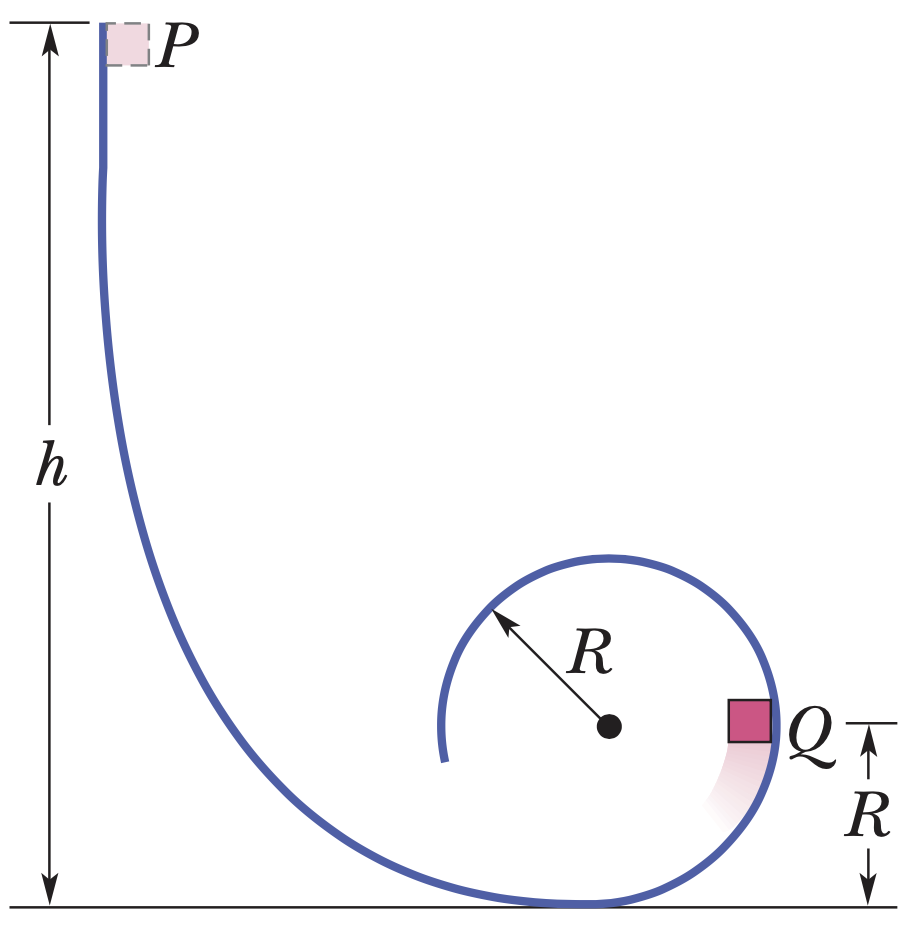
\includegraphics[scale=0.3]{Qfig8-3-20220328.png}
  \caption{문제 3}
  \label{fig:3}
\end{figure}
토막이 점 $P$에서
\begin{itemize}
\item[(가)] 점 $Q$
\item[(나)] 트랙의 꼭대기에 도달했을 때 중력이 토막에 한 일은 각각
  얼마인가?
\end{itemize}
트랙의 바닥에서 토막-지구 계의 중력 퍼텐셜 에너지를 $0$으로 하면 
\begin{itemize}
\item[(다)] 점 $P$
\item[(라)] 점 $Q$
\item[(마)] 트랙의 꼭대기에서의 중력 퍼텐셜에너지는 각각 얼마인가?
\item[(바)] 단순히 토막을 놓지 않고 일정 속력을 주어 토막을 아래로
  밀었다면 (가)에서 (마)까지의 답은 각각 증가, 감소, 불변 중 어느
  것인가? 
\end{itemize}
\newpage

{\color{gray} [문제 풀이 쪽]}

\newpage

\end{document}